\chapter{Листинги программного кода}\label{app:A}

\section{Функция трассировки луча через систему зеркал}\label{app:A1}

\begin{ListingEnv}[!h]% настройки floating аналогичны окружению figure
\captiondelim{ } % разделитель идентификатора с номером от наименования
\caption{Листинг функции трассировки луча через систему зеркал}\label{lst:beam_trace}
% окружение учитывает пробелы и табуляции и применяет их в сответсвии с настройками

Функция $trace\_beam$ \ref{lst:beam_trace} позволяет получить центр и волновой вектор при прохождении луча через систему зеркал. Так как при трассировке луча отражения рассматриваются последовательно и независимо друг от друга, то данную функцию легко для любого геометрического расположения зеркал в различных конфигурациях интерферометра.  


\begin{lstlisting}[language=Python]
def trace_beam(self, mirror1_normal, mirror2_normal):
    # initial center and wave_vector
    center = np.array(
        [0, -self.a, -(self.b + self.c)]
    )
    wave_vector = np.array([0, 0, 1])

    # reflect beam by first mirror
    center = project(
        center, wave_vector, 
        mirror1_normal, np.array([0, -self.a, -self.c])
    )
    wave_vector = reflect(wave_vector, mirror1_normal)

    # reflect beam by second mirror
    center = project(
        center, wave_vector, 
        mirror2_normal, np.array([0, 0, -self.c])
    )
    wave_vector = reflect(wave_vector2, mirror2_normal)

    return center, wave_vector
\end{lstlisting}
\end{ListingEnv}

\section{Функция рассчитывающая параметры луча при прохождении системы зеркал}\label{app:A2}

\begin{ListingEnv}[!h]
\captiondelim{ }
\caption{Функция рассчитывающая параметры луча при прохождении системы зеркал}\label{lst:beam_propag}

\begin{lstlisting}[language=Python]
def propagate_beam(self, lens_dist):
    if lens_dist == 0:
        lens_dist = 1e-6

    # ABCD matrix for free space
    def free_space(length):
        return np.array([[1, length], [0, 1]])

    # ABCD matrix for a lens
    def lens(focal_length):
        return np.array([[1, 0], [-1 / focal_length, 1]])

    dist_between_lenses = self.f1 + self.f2 + lens_dist

    dist_to_camera = self.c + self.a + self.b - dist_between_lenses
    
    # compute ABCD matrix 
    abcd_matrix = \
        free_space(dist_to_camera) @ \
        lens(self.f2) @ \
        free_space(dist_between_lenses) @ \
        lens(self.f1)
    
    # compute parameter q
    inv_q = -1j * self.lamb / (np.pi * self.radius ** 2)
    inv_q_prime = (abcd_matrix[1][0] + abcd_matrix[1][1] * inv_q) / (abcd_matrix[0][0] + abcd_matrix[0][1] * inv_q)

    curvature_radius = 1 / (np.real(inv_q_prime) + 1e-9)
    beam_radius = np.sqrt(-self.lamb / np.imag(inv_q_prime) / np.pi)
    
    return beam_radius, curvature_radius
\end{lstlisting}
\end{ListingEnv}

Функция $propagate\_beam$ \ref{lst:beam_propag} рассчитывает радиус кривизны волнового фронта и радиус пучка после прохождения плеча интерферометра. Расчет производится на основании $ABCD$-матрицы составленной на основании используемых в интерферометре оптических элементов. Функция $propagate\_beam$ также может быть легко адаптирована к изменению расположения и изменению количества используемых оптических элементов. 

\FloatBarrier


\section{Листинг функции вычисления интерференционной картины}\label{app:A3}

Функция $calcImage$ \ref{lst:calcImage} рассчитывает интерференционную картину при заданных параметрах двух интерферирующих лучей. 

%\begin{ListingEnv}[!h]% настройки floating аналогичны окружению figure
\captiondelim{ } % разделитель идентификатора с номером от наименования
%\caption{Листинг функции вычисления интерференционной картины}\label{lst:beam_trace}
% окружение учитывает пробелы и табуляции и применяет их в сответсвии с настройками
\begin{lstlisting}[language=C++,tabsize=4,label={lst:calcImage},caption={Листинг функции вычисления интерференционной картины}]
void calcImage(
		double xstart, double ystart, 
		int xpoints, int ypoints, double pixel_size,
		const Vector& wave_vector1, const Vector& center1, 
		double radius1, double beam1Ampl,
        const Vector& wave_vector2, const Vector& center2, 
        double radius2, double beam2Ampl, 
        double r_curvature, int nForwardFrames, 
        int nBackwardFrames, double lambda, double omega, 
        double noiseCoeff, double amplStd, double phaseStd,
        int nThreads, uint8_t* image, double* totIntens) {
    auto calcIntens = [&](double a1, double a2, double deltaPhi) {
        const auto i1 = a1 * a1;
        const auto i2 = a2 * a2;
        return i1 + i2 + 2 * a1 * a2 * cos(deltaPhi);
    };

    const int totalPoints = xpoints * ypoints;
    std::vector<double> ampl1(totalPoints);
    std::vector<double> ampl2(totalPoints);
    std::vector<double> deltaPhase(totalPoints);

    auto worker = [&](int kStart, int kEnd) {
        for (int k = kStart; k < kEnd; ++k) {
		    int i = k / ypoints;
		    int j = k % ypoints;
		    const Vector point = {xstart + i * pixel_size, ystart + j * pixel_size, 0};

            const Vector source2 = utils::backTrack(point, wave_vector2, center2);
            const double dist2 = utils::dist(point, source2);
            auto w2 = calcWave2(dist2, source2[0], source2[1]);

            const Vector source1 = utils::backTrack(point, wave_vector1, center1);
            const double dist1 = utils::dist(point, source1);
	        auto w1 = calcWave1(dist1, source1[0], source1[1]);
	        
            ampl1[k] = w1.ampl;
            ampl2[k] = w2.ampl;
            deltaPhase[k] = w1.phase - w2.phase;
		}
	};

	const int pointsPerThread = totalPoints / nThreads;
	std::vector<std::future<void>> futures;

	for (int iThread = 0; iThread < nThreads; ++iThread) {
		int kStart = pointsPerThread * iThread;
		int kEnd = kStart + pointsPerThread;
		futures.push_back(std::async(std::launch::async, worker, kStart, kEnd));
	}

    // wait for intens1, intens2, deltaPhase
	for (const auto& f : futures) {
		f.wait();
	}

    auto imageWorker = [&](uint8_t* img, double time, double& integIntens) {
        for (int k = 0; k < totalPoints; ++k) {
            const double intens = calcIntens(
                ampl1[k], 
                ampl2[k], 
                deltaPhase[k] - omega * time
            );
            const double rescaledIntens = std::min(intens / maxIntens, 1.0);
            const double intensWithNoise = (rescaledIntens + noise()) / (1 + noiseCoeff);
            img[k] = static_cast<uint8_t>(255 * intensWithNoise);
            integIntens += intens;
        }
    };

    std::vector<std::future<void>> imageFutures;

    auto startPhase = rndPhase();
    for (int iFrame = 0; iFrame < nForwardFrames; ++iFrame) {
        double time = startPhase + 2 * M_PI * iFrame / nForwardFrames + piezoNoise();
        int ind = iFrame * totalPoints;
        uint8_t* img = image + ind;
        imageFutures.push_back(std::async(
            std::launch::async, imageWorker, img, time,
            std::ref(totIntens[iFrame])));
    }

    startPhase = rndPhase();
    for (int iFrame = 0; iFrame < nBackwardFrames; ++iFrame) {
        double time = startPhase + 2 * M_PI * (1.0 - static_cast<double>(iFrame) / nBackwardFrames) + piezoNoise();
        int ind = (iFrame + nForwardFrames) * totalPoints;
        uint8_t* img = image + ind;
        imageFutures.push_back(std::async(
            std::launch::async, imageWorker, img, time,
            std::ref(totIntens[iFrame + nForwardFrames])));
    }

    // wait for frames
    for (const auto& f : imageFutures) {
        f.wait();
    }
}
\end{lstlisting}
%\end{ListingEnv}

\section{Листинг задания нейронной сети DQN агента}\label{app:A4}

\begin{ListingEnv}[!h]
\captiondelim{ }
\caption{Нейронная сеть DQN агента}\label{lst:dqn}

\begin{lstlisting}[language=Python]

class DuelDQNModel(nn.Module):
    def __init__(self, inpshape, n_actions):
        super(DuelDQNModel, self).__init__()
        
        self.conv = nn.Sequential(
            nn.Conv2d(inpshape[0], 32, kernel_size=8, stride=4),
            nn.ReLU(),
            nn.Conv2d(32, 64, kernel_size=4, stride=2),
            nn.ReLU(),
            nn.Conv2d(64, 64, kernel_size=3, stride=1),
            nn.ReLU()
        )
        conv_out_size = get_out(inpshape, self.conv)

        self.fc_adv = nn.Sequential(
            nn.Linear(conv_out_size, 512),
            nn.ReLU(),
            nn.Linear(512, 512),
            nn.ReLU(),
            nn.Linear(512, n_actions)
        )
        self.fc_val = nn.Sequential(
            nn.Linear(conv_out_size, 512),
            nn.ReLU(),
            nn.Linear(512, 512),
            nn.ReLU(),
            nn.Linear(512, 1)
        )

    def forward(self, x, histo):
        x = x.float() / 255.0
        conv_out = self.conv(x).view(x.shape[0], -1)
        val = self.fc_val(conv_out)
        adv = self.fc_adv(conv_out)
        return val + adv - adv.mean()
\end{lstlisting}
\end{ListingEnv}

\section{Листинг задания нейронной сети TD3 агента}\label{app:A5}

\begin{ListingEnv}[!h]
\captiondelim{ }
\caption{Нейронная сеть TD3 агента}\label{lst:td3}

\begin{lstlisting}[language=Python]

class TD3Actor(nn.Module):
    def __init__(self, state_dim, action_dim, hid_dim):
        super(Actor, self).__init__()
        self.vgg16 = nn.Sequential(
            nn.Conv2d(16, 32, kernel_size=3, padding=1)
            nn.ReLU(),
            nn.Conv2d(32, 32, kernel_size=3, padding=1)
            nn.ReLU(),
            nn.MaxPool2d(2, 2), 
            nn.Conv2d(32, 64, kernel_size=3, padding=1)
            nn.ReLU(),
            nn.Conv2d(64, 64, kernel_size=3, padding=1)
            nn.ReLU(),
            nn.MaxPool2d(2, 2), 
            nn.Conv2d(64, 128, kernel_size=3, padding=1)
            nn.ReLU(),
            nn.Conv2d(128, 128, kernel_size=3, padding=1)
            nn.ReLU(),
            nn.MaxPool2d(2, 2), 
            nn.Conv2d(128, 256, kernel_size=3, padding=1)
            nn.ReLU(),
            nn.Conv2d(256, 256, kernel_size=3, padding=1)
            nn.ReLU(),
            nn.MaxPool2d(2, 2),
            nn.Flatten()
        )
        self.mlp = nn.Sequential(
            nn.Linear(get_out(self.vgg16, state_dim), hid_dim),
            nn.ReLU(),
            nn.Linear(hid_dim, hid_dim),
            nn.ReLU(),
            nn.Linear(hid_dim, action_dim),
            nn.Tanh()
        )
\end{lstlisting}
\end{ListingEnv}    


\chapter{Вывод основных формул}\label{app:B}

\section{Вывод формулы видности для интерферометра Маха-Цендера (\ref{eq:visib_rot})}\label{app:B1}

Для вычисления видности интерференционной картины в соответствии с уравнением~(\ref{eq:visib}), вычислим суммарную интенсивность света в плоскости камеры($z=0$):

\begin{align}
    I(t)&=\int |E_1(x,y,0,t)+E_2(x,y,0,t)e^{i\phi_{\mathrm{piezo}}(t)}|^2 {\mathrm{d}}x{\mathrm{d}}y \nonumber \\
    &= \int \left[E_1 E_1 ^* + E_2 E_2^* + E_1 E_2^*e^{i\phi_{\mathrm{piezo}}(t)} + E_1^*E_2e^{i\phi_{\mathrm{piezo}}(t)}\right]{\mathrm{ d}}x{\mathrm{d}}y ,\label{eq:itot}
\end{align}
где амплитуды индивидуальных лучей определяются уравнением~(\ref{eq:Exyzt}):

\begin{align*}
    E_1(x,y,0,t) &=\exp\left[-\frac{(x-x_0)^2}{r^2}\right] \exp(i k_x(x - x_0)) \cdot \exp\left[-\frac{(y-y_0)^2}{r^2}\right] \exp(i k_y(y - y_0));\\
   E_2(x,y,0,t) &=\exp\left[-\frac{x^2}{r^2}\right] \cdot \exp\left[-\frac{y^2}{r^2}\right].
\end{align*}

С помощью табличного интеграла $\Int \exp(-\frac{ax^2}{2} + i Jx) {\mathrm{d}} x= \left(\frac{2\pi}{a}\right)^{1/2} \cdot \exp(-\frac{J^2}{2a})$, вычислим первые два слагаемых в уравнении~(\ref{eq:itot}),

\begin{multline}
\Int \left(E_1 E_1^* + E_2 E_2^*\right){\mathrm{d}}x{\mathrm{d}}y = \\
2 \Int \exp\left(-\frac{2x^2}{r^2}\right){\mathrm{d}}x \cdot \Int \exp\left(-\frac{2y^2}{r^2}\right){\mathrm{d}}y = \pi r^2,
\label{eq:itot_1}
\end{multline}

Далее найдем оставшиеся два слагаемых:

\begin{multline}
\Int \left(E_1 E_2^* + E_1^* E_2 \right) {\mathrm{d}}x{\mathrm{d}}y =\\ \pi r^2 \exp\left[-\frac{(k_x^2 + k_y^2)r^2}{8}\right] \exp\left(-\frac{x_0^2 + y_0^2}{2r^2}\right) \cos\left(\frac{k_x x_0 + k_y y_0}{2} -\phi_{\mathrm{piezo}}(t)\right)
\label{eq:itot_2}
\end{multline}

Просуммируем уравнение~(\ref{eq:itot_1}) и (\ref{eq:itot_2}), получим

\begin{multline}
I_{\mathrm{tot}}(t) = \pi r^2 \biggl[1 +  \exp\left(-\frac{(k_x^2 + k_y^2)r^2}{8}\right) \exp\left(-\frac{x_0^2 + y_0^2}{2r^2}\right)\cdot \\ \cos\left(\frac{k_x x_0 + k_y y_0}{2} -\phi_{\mathrm{ piezo}}(t)\right)\biggr]
\end{multline}

Далее подставим полученное выражение для $I_{\mathrm{tot}}(t)$ в уравнение~(\ref{eq:visib}), учитывая что максимум и минимум $I_{\mathrm{tot}}(t)$ соответствует $\cos(\cdot) = \pm 1$, получим уравнение~(\ref{eq:visib_rot}).


\section{Вывод формулы видности для интерферометра Маха-Цендера с линзами (\ref{eq:visib_lense})}\label{app:B2}

Рассмотрим как изменяются параметры пучка при нормальном падении на систему линз. Первоначально пучок имеет плоский волновой фронт ($\rho \to \infty$). В соответствии с уравнениями \eqref{eq:abcd_free}, \eqref{eq:abcd_lens}, \eqref{eq:abcd_prod} матрица $M$ для системы из линзы с фокусным расстоянием $F_{1}$, вакуума длинной $F_{1} + F_{2} + \Delta$, линзы $F_{2}$ и вакуума длинной $d$ равна:

\begin{equation*}
M =
\begin{pmatrix}
 \dfrac{d\Delta - F_{2}^2 - \Delta F_{2}}{F_{1}F_{2}} & \dfrac{F_{1}F_{2} + F_{2}^2 + \Delta F_{2} - F_{1}d- \Delta d}{F_{2}} \\
\dfrac{\Delta}{F_{1} F_{2}} & - \dfrac{F_{1} + \Delta}{F_{2}} \\
\end{pmatrix}
\end{equation*}

Изначально считаем, что волна является плоской ($\rho \to \infty$), а значит параметр $q$ \eqref{eq:q_param} равен:

\begin{equation*}
    \dfrac{1}{q} = - \dfrac{i \lambda}{\pi r^2}
\end{equation*}

Из формулы \eqref{eq:q_prime} разделив числитель и знаменатель на $q$, затем умножив числитель и знаменатель на $F_{1} F_{2}$, и получим:

\begin{equation*}
    q' = \dfrac{(d\Delta - F_{2}^2 - \Delta F_{2}) - F_{1}(F_{1}F_{2} + F_{2}^2 + \Delta F_{2} - F_{1}d- \Delta d)\dfrac{i \lambda}{\pi r^2}}{\Delta + F_{1}(F_{1} + \Delta) \dfrac{i \lambda}{\pi r^2}} 
\end{equation*}

Соответственно:

\begin{equation}
    \dfrac{1}{q'}= \dfrac{1}{(d\Delta - F_{2}^2 -\Delta F_{2})^2} \Big((d\Delta - F_{2}^2 - \Delta F_{2})\Delta - F^{2}_{1}F^{2}_{2}\dfrac{i \lambda}{\pi r^2}\Big)
\label{eq:inv_q_prime}
\end{equation}

Выражение \eqref{eq:inv_q_prime} получено в приближении  $\Delta \ll F^3 \dfrac{ \lambda^2}{\pi^2 r^4}$, где $\Delta$ --- шаг микрометрического винта. Из выражения \eqref{eq:inv_q_prime} получим уравнения для радиуса кривизны волнового фронта и радиуса пучка: 

\begin{equation}
    \rho ' =  \dfrac{d\Delta - F_{2}^2 - \Delta F_{2}}{\Delta}
\end{equation}

\begin{equation}
    r' = \Big |\dfrac{d\Delta}{F_{1}F_{2}} - \dfrac{F_{2}}{F_{1}} - \dfrac{\Delta}{F_{1}}\Big|r
\end{equation}

Далее видность рассчитывается в соответствии с уравнениями \eqref{eq:I_def}, \eqref{eq:visib}, где интенсивности пучков заданы уравнениями \eqref{eq:upper_beam}, \eqref{eq:lower_beam}. Итоговое выражение для видности интерференционной картины получается следующим:

\begin{equation}
\begin{split}
    V =\frac{4}{\left(n^{2}+1\right) r^{2}} \frac{1}{c} \exp \left(-\left(x_{0}^{2}+y_{0}^{2}\right)\left(\frac{1}{r^{2} n^{2}}-\frac{n^{2}+1}{n^{6} r^{6} c^{2}}\right)\right) \times \\ \times \exp \left(-\frac{n^{2}+1}{4 c^{2} n^{2} r^{2}}\left(k_{x}^{2}+k_{y}^{2}\right)\right) \exp \left(\frac{\frac{\pi}{\lambda \rho^{\prime}}}{n^{2} r^{2} c^{2}}\left(x_{0} k_{x}+y_{0} k_{y}\right)\right),
\end{split}
\end{equation}
где параметр $n=\dfrac{r^{\prime}}{r}$ и параметр $c^2 = (\dfrac{n^2 + 1}{n^2r^2})^2$.

\chapter{Изображения интерференционных картин}\label{app:C}

\begin{figure}[ht]
\centerfloat{
        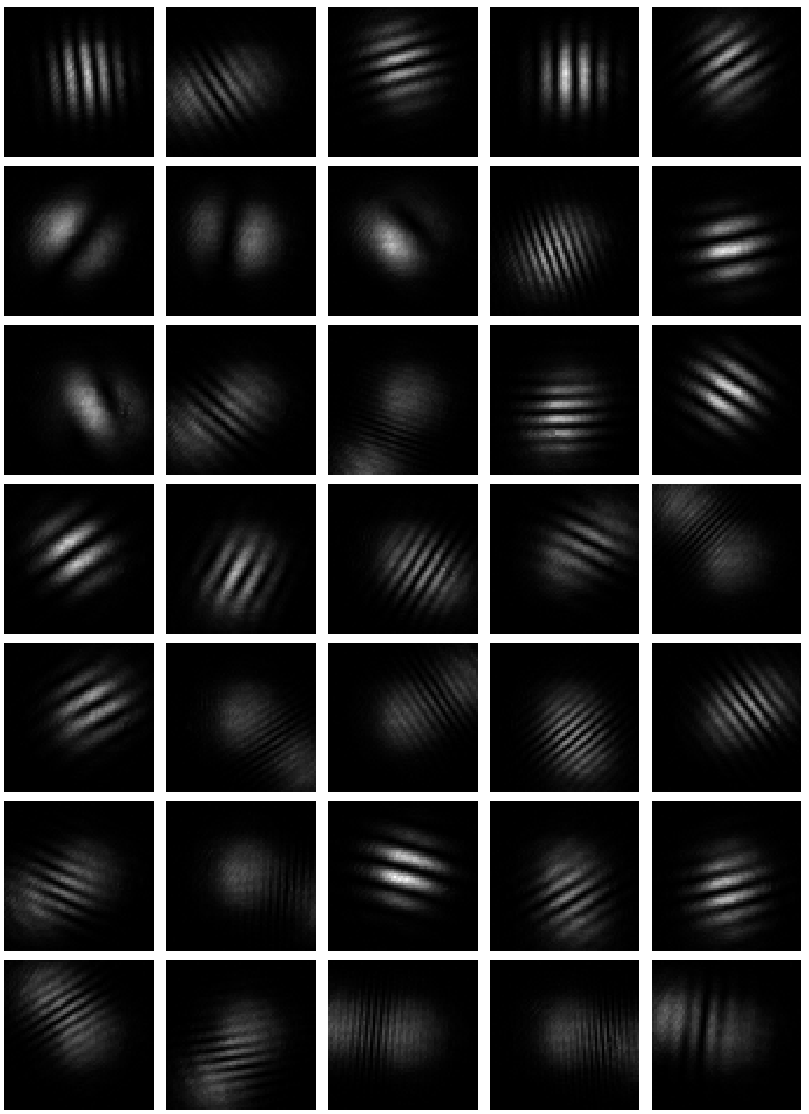
\includegraphics[width=0.75\textwidth]{images/interf_patterns.pdf}
}
\caption{Примеры интерференционных картин наблюдаемые при настройке оптического интерферометра Маха-Цендера.}
    \label{fig:interf_patterns}
\end{figure}


\clearpage
%\refstepcounter{chapter}
%\addcontentsline{toc}{appendix}{\protect\chapternumberline{\thechapter}Чертёж детали}

%\includepdf[pages=-]{Dissertation/images/drawing.pdf}
